\subsection{Steps to use Overleaf with Jupyter
notebook}\label{steps-to-use-overleaf-with-jupyter-notebook}

The steps were as follows:

\begin{enumerate}
\def\labelenumi{\arabic{enumi}.}
\tightlist
\item
  We created an article in Overleaf first
\item
  We then pushed the article to github
\item
  We visited github and copied the address of the article that we'd
  clone
\item
  We then created a new git repository on our machine where we have
  cloned the directory (in our case, we called that ``work'')
\end{enumerate}

Now,

\begin{itemize}
\tightlist
\item
  We have added a jupyter notebook
\item
  The jupyter notebook will let us add text using markdown documentation
\item
  We will continue to store our bibliography information on the
  references.bib file in bibtex format
\item
  We will add citation information using
  \texttt{\textbackslash{}cite\{citationid\}}
\end{itemize}

\subsection{Next Steps}\label{next-steps}

We will convert this notebook to latex using two steps: In the first
step, we will convert the notebook to a markdown file, using

\texttt{jupyter\ nbconvert\ test\_section.ipynb} This will convert this
notebook to markdown format. Then we will convert the test\_section.md
to test\_section.tex using pandoc as

\texttt{pandoce\ -f\ markdown\ -t\ latex\ -o\ test\_section.tex\ test\_section.md}

We will then do some more things:

\begin{enumerate}
\def\labelenumi{\arabic{enumi}.}
\tightlist
\item
  We will create .gitignore file that will contain all files with
  extension \texttt{*.ipynb} as git as problems in maintaining them.
\item
  Optionally, if we do not want to share our markdown files, we will add
  \texttt{*.md} files to the list as well.
\item
  Lastly, and optionally, we can add the new \texttt{test\_section.tex}
  file to the \texttt{main.tex} file using the
  \texttt{\textbackslash{}input\{test\_section\}}
\end{enumerate}

After we have done these three changes, we will then push the files to
the git repo using:

\begin{verbatim}
git pull origin master
git add test_section.tex main.tex
git commit -m "added test_section files"
git push origin master
\end{verbatim}

Then, once we are in Overleaf, we will pull in the changes to Overleaf
and work on Overleaf.

Once you are in Overleaf, you can edit the document and continue to push
to github. Each file that you push to github will then be pulled into
the computer of your collaborators or your own computer (depending on
where you have been working). You can work on a minimal computer that
gets connected to the web or a not compatible operating system that can
connect to the web and you can use a hosted instance of jupyter notebook
where you can work. If that is the case, then you can use the hosted
instance to work on the returned or received document and work on it. If
you are familiar with latex, then you can directly continue to work on
the document in a jupyter notebook environment and push the changes back
to overleaf. If you are happy to work with markdown, then you contine to
convert the latex file from latex to markdown and work directly on the
markdown document and remember to reconvert and push to Overleaf. If you
want to continue to work on the test\_section.ipynb, you can do so, but
this time when you export to latex, save it with a different name or
something like version 2 or somehow that signifies that this file is
different from the previous one that you sent. This way, going back and
forth, you can combine powerful and weak machines, web and offline, in
many different ways to set up a workflow that pulls and pushes changes
to the flow of your work.

The result will be a pdf document (only on Overleaf), but if you want,
you can use pandoc at your end to convert the document (or the latex
document that results from Overleaf) to word document and continue to
publish for those situations where a word document is desired. I
recommend that you start with an article template that Overleaf provides
rather than open a blank article as this helps you to get things done
quickly.

\begin{Shaded}
\begin{Highlighting}[]
\CommentTok{# let's say now we want to analyse some data in R and write our paper}
\KeywordTok{library}\NormalTok{(tidyverse)}
\KeywordTok{library}\NormalTok{(ggplot2)}
\KeywordTok{data}\NormalTok{(mtcars)}
\NormalTok{mtcars }\OperatorTok
\StringTok{  }\KeywordTok{ggplot}\NormalTok{() }\OperatorTok{+}
\StringTok{  }\KeywordTok{geom_bar}\NormalTok{(}\KeywordTok{aes}\NormalTok{(}\DataTypeTok{x =}\NormalTok{ gear)) }\OperatorTok{+}
\StringTok{  }
\StringTok{  }\KeywordTok{ggtitle}\NormalTok{(}\StringTok{"Gear types"}\NormalTok{)}
  
\end{Highlighting}
\end{Shaded}

\begin{figure}
\centering
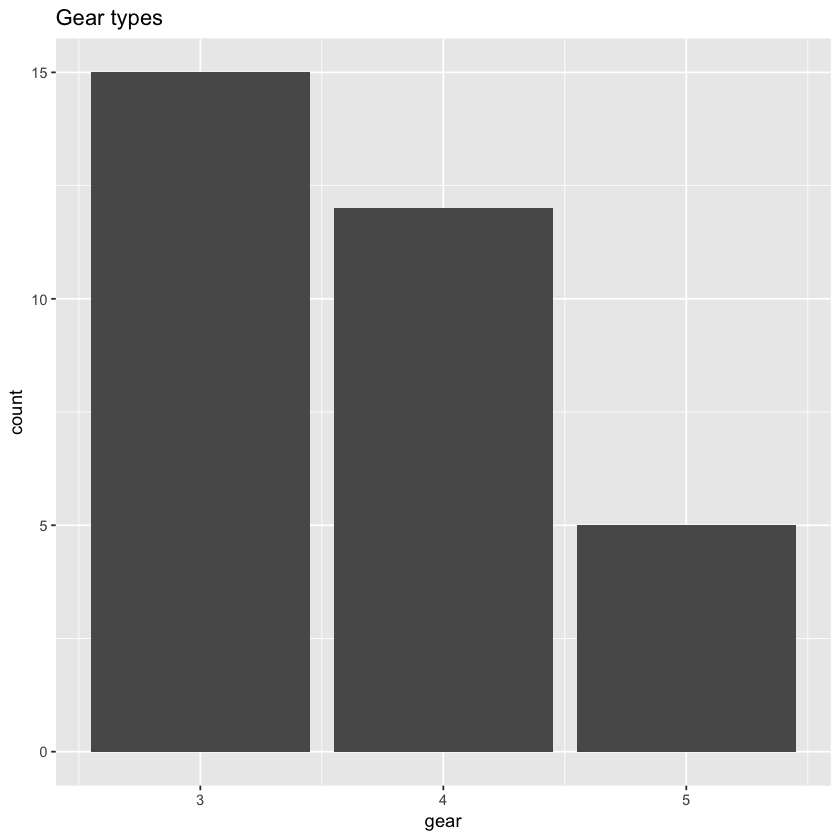
\includegraphics{test_section_files/test_section_2_1.png}
\caption{png}
\end{figure}
